Nachdem die Implementation der 2D-DFT in VHDL erfolgt ist, werden anhand von Simulationen und eines selbstgeschriebenen Skripts Testdurchläufe durchgeführt, die die
korrekte Berechnung überprüfen.
Daran schließt sich die Chipimplementation an, bei der die Gatter in vorm von Standarzellen des Auftragsfertigers \gls{ams} auf dem Chip platziert werden.

\section{Simulation der 2D-DFT}
Zur Simulation von Hardwarekomponenten dient in der Cadence-Umgebung das Programm NC\,Sim. Damit die Signalverläufe grafisch dargestellt werden, wird aus NC\,Sim 
heraus SimVision gestartet.
Es ermöglicht das Betrachten der Signalzustände, die im Top-Modul als externes Signal in der Entity (Eingang oder Ausgang einer Komponente) sowie internes Signal 
(\texttt{signal}) deklariert wurden. Wenn in der Top Level Entity instanziierte Komponenten untereinander verbunden sein sollen, müssen entsprechende Signale 
deklariert und ihnen zugewiesen werden. Diese Signale sind deshalb in der Simulation auch zu sehen. Signale die innerhalb einer eingebetteten Komponente verwendung finden, sind 
nicht sichtbar und müssen gegebenfalls zumindest temporär zusätzlich als Ausgang der Komponente hinzugefügt werden.
Das Programm beherrscht lediglich bei einzelnen Vektoren die Umrechnung zu vorzeichenbehafteten Zahlen im Dezimalsystem.
Bei der Bündelung von Vektoren können nur positive Dezimalzahlen dargestellt werden. Dies hat zur Folge, dass Vektoren, die eine negative Zahl repräsentieren, 
bei Bedarf händisch umgerechnet werden müssen. 
Erfolgen kann das mittels $2^{n+1}+m$, $n=$ Bitbreite des Vektors und $m=$ angezeigte Zahl. Die Darstellung von Festkommazahlen ist in keinem Fall möglich.

 Anhand der Simulation kann die Anzahl der im Voraus ermittelten, zur Berechnung der 2D-DFT benötigten Takte, verifiziert werden, was nachfolgend geschehen soll.
 
 Nachdem \texttt{nReset} auf '1' gesetzt wird, werden die Eingangswerte
 eingelesen. Wenn dieser Vorgang abgeschlossen ist, geht \texttt{loaded} auf '1'. Mit der nächsten steigenden Taktflanke, in Bild \ref{pic:Simulationsdauer} bei 
 \SI{340}{ns}, beginnt die Berechnung
 der \gls{2d-dft}. Beendet ist sie, nachdem die Matrizenmultiplikation auf die Eingangswerte und anschließend auf die \gls{1d-dft}-Werte angewandt wurde. Also nach $2 \cdot 64$
 einzelnen Berechnungen. Wenn dies erfolgt ist, wird \texttt{result\_ready} auf '1' gesetzt. Dies geschieht bei \SI{20\,820}{ns}. Bei einer Taktfrequenz von $(\SI{40}{ns})^{-1}$
 (siehe \ref{src:dft8_optimiert_top}) ergeben sich so 512 Takte. Dies bestätigt auch der Edge Count, ebenfalls auf dem Bild zu sehen, welcher die Flanken des \texttt{clk}-Signals 
 zählt. In der Simulation ist zu erkennen, dass die Berechnung der Elemente 
 unterschiedlich viele Takte beansprucht. Hieran lässt sich ebenfalls sehen, dass die 1. (ungerade) Zeile weniger Takte gegenüber der 2. (geraden) Zeile benötigt. 
 
 %Auch in der Abbildung \ref{pic:Simulationsdauer} zu sehen ist, dass \texttt{element\_out} für 0 bis 7 weniger Takte einnimmt, als in den darauf folgenden 8. Dieses Muster
 %wiederholt sich und hat, wie in Abschnitt \ref{sec:berechnung_anzahl_takte} erläutert, damit zu tun, dass für die geraden
 
 \begin{figure}[htbp]
  \centering
  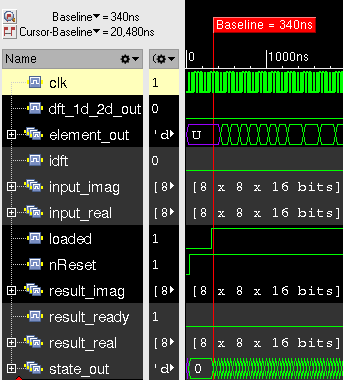
\includegraphics[width=0.58\textwidth]{img/Simulationsdauer_Anfang.png}
  \hfill
  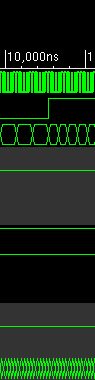
\includegraphics[width=0.161\textwidth]{img/Simulationsdauer_Mitte.png}
  \hfill
  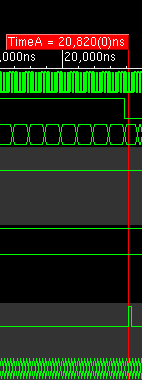
\includegraphics[width=0.241\textwidth]{img/Simulationsdauer_Ende.png}
  \caption{Ausschnitt des Simulationstools \texttt{NC\,Sim} von der Berechnung und Verifikation der 2D-DFT.}
  \label{pic:Simulationsdauer}
 \end{figure}

 \begin{figure}[htbp]
  \centering
  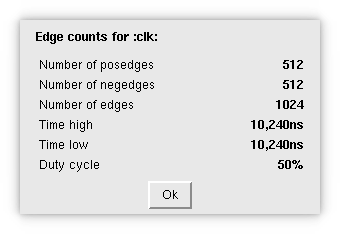
\includegraphics[width=0.6\textwidth]{img/Simulation_edge_count_clk.png}
  \caption{Edge Count des Taktsignals für die vollständige Simulation der 2D-DFT.}
 \end{figure}




 